% Third Workshop on AI in Production @ KI 2026
% CEUR-WS format — Full/Position Paper (up to 10 pages)
\documentclass[]{ceurart}

\sloppy

\usepackage{amsmath}
\usepackage{booktabs}
\usepackage{xcolor}
\usepackage{graphicx}

\begin{document}

\copyrightyear{2026}
\copyrightclause{Copyright for this paper by its authors.
  Use permitted under Creative Commons License Attribution 4.0
  International (CC BY 4.0).}

\conference{FGWM 2026: Workshop of the GI Special Interest Group on
  Knowledge Management, August 11--12, 2026, Bremen, Germany}

\title{From Documentation to Knowledge Vessels:\\Agentic AI for Tacit
  Knowledge Preservation in Manufacturing}

\author{Michael Banf}[%
  email=michael.banf@perelyn.com,
]
\cormark[1]
\author{Johannes Kuhn}

\author{Dominik Filipiak}

\author{Max Becker}

\author{Sebastian Fetz}

\address{Perelyn GmbH, Munich, Germany}

\cortext[1]{Corresponding author.}

\begin{abstract}
Manufacturing faces an unprecedented knowledge crisis: an estimated 70\%
of critical operational expertise is undocumented and resides in aging
workers' heads. Current AI-based knowledge capture treats this as a
documentation problem, resulting in extracting expertise into static SOPs,
knowledge graphs, or video tutorials. In this position paper, we argue
for a fundamental reframing, i.e. tacit knowledge preservation should be
understood as an agent memory problem. Drawing on a landscape
analysis of commercial platforms and agentic memory research,
we identify a critical episodic-temporal gap. No existing system
captures the situated, evolving, episode-grounded nature of expert
knowledge. We sketch a three-stage
architecture, \textsc{Capture}--\textsc{Organize}--\textsc{Transfer}, in
which graph-based memory structures, including episode graphs, knowledge graphs, and 
procedure trees, serve as the unifying representation at every layer,
enabling agentic AI to incrementally absorb, structure, and deliver
expertise as persistent knowledge vessels. Rather than presenting
a finished implementation, we lay out this architectural vision as an invitation
to the community to discuss the design space, identify overlooked
challenges, and collaboratively advance memory-grounded knowledge
preservation in manufacturing.
\end{abstract}

\begin{keywords}
  Tacit knowledge \sep
  Manufacturing \sep
  Agentic AI \sep
  Knowledge preservation \sep
  Agent memory \sep
  Multimodal capture
\end{keywords}

\maketitle

%%% ==================================================================
\section{Introduction}\label{sec:intro}
%%% ==================================================================

The manufacturing sector confronts a structural knowledge crisis driven
by workforce demographics. In the United States, 52.4\% of the
industrial products workforce is expected to retire or depart within
five years~\cite{apqc2025}, creating an estimated 2.8~million
retirement-driven vacancies by 2033~\cite{deloitte2024}. The average age
in small manufacturing shops approaches~55, with ownership often in
their 60s~\cite{edwards2026}. Each retiring technician with 20+ years of
experience takes approximately \$800K--\$1.2M in undocumented
troubleshooting knowledge~\cite{dovient2025}. Fortune warned in
January 2026 that there are an estimated 1--2 years left to capture
decades of industrial knowledge~\cite{fortune2026}. An estimated 70\% of
critical manufacturing knowledge is never
formalized~\cite{egain2025}, and knowledge transfer failures cost large
manufacturers \$47~million per year~\cite{panopto2018}. When tribal
knowledge is lost, repair times increase 3--4$\times$ and new-hire
ramp-up extends from 3--4 months to 8--12~months~\cite{dovient2025}. The crisis is equally acute in Europe. In Germany, 13.4~million
workers, i.e. 31\% of the labor force, will exceed the legal retirement age
by 2039~\cite{destatis2025}. The Babyboomer cohort (16.5~million)
outstrips incoming workers (12.5~million) by four million, creating an
irreversible demographic gap~\cite{iwkoeln2025}. In the skilled trades, 125,000 businesses face generational succession
within five years and 80,000 craft jobs were lost in 2024 alone because
owners found no successors~\cite{zdh2025}. Critically, 57\% of non-fillable positions are in
dual-vocational-training occupations~\cite{dihk2025}, which are precisely the roles where tacit
knowledge is most concentrated. Yet only 17\% of German manufacturing
companies actively deploy AI~\cite{bitkom2026}, revealing a paradox, i.e. the
German Mittelstand is simultaneously the most affected by tacit knowledge
loss and the least equipped with AI tools to address it.

A rapidly growing ecosystem of commercial platforms and academic
prototypes has emerged to address this crisis. Yet virtually all treat
tacit knowledge preservation as a documentation problem, which means conducting
interviews, recording SOPs, transcribing video, and storing results as static
artifacts. This framing discards the very qualities that make expert
knowledge valuable, i.e. its situatedness, temporal evolution, and
episode-grounded nature.

We propose a conceptual reframing of tacit
knowledge preservation not as a documentation problem but as an
agent memory problem. Recent surveys reveal that all major agent
harnesses lack episodic memory and temporal
versioning~\cite{hu2025survey}, precisely the capabilities needed to
capture how expert knowledge is situated, evolves over time, and is
grounded in specific episodes. This reframing is not merely semantic; it
shifts the design space from static capture-and-store pipelines to
living memory architectures that continuously absorb, structure,
and deliver expertise, even long after the original expert has retired.

\begin{table}[t]
\centering
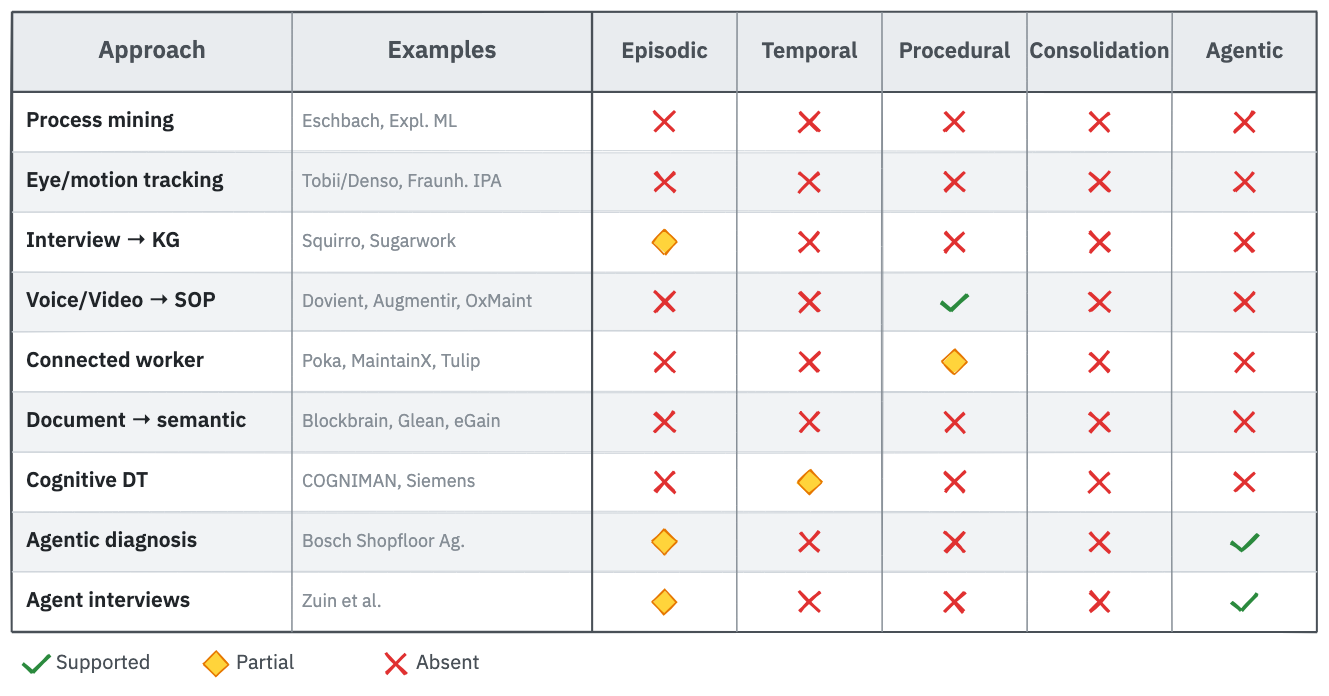
\includegraphics[width=\textwidth]{figures/tacit-landscape-table.png}
\caption{Feature matrix of knowledge capture approaches assessed against
  five memory capabilities, including episodic, temporal, procedural,
  consolidation, and agentic, derived from the CoALA taxonomy and the
  bi-temporal model. No surveyed system achieves more than two of five
  capabilities.}\label{tab:landscape}
\end{table}

We sketch a three-stage architecture, labelled \textsc{Capture}--\textsc{Organize}--\textsc{Transfer}, and argue that
graph-based representations, including episode graphs, knowledge graphs,
procedure trees, provide the natural unifying substrate at every layer.
Rather than reporting a completed system, this paper lays out the
architectural vision and invites the community to discuss its
feasibility, identify blind spots, and collaborate on realizing
memory-grounded knowledge preservation in manufacturing.

%%% ==================================================================
\section{Current Landscape}\label{sec:landscape}
%%% ==================================================================

We surveyed the current landscape of AI-based tacit knowledge
preservation in manufacturing across commercial platforms, academic
prototypes, and industry initiatives. At least 17 commercial products now target manufacturing knowledge
capture, from dedicated startups, including Dovient~\cite{dovient2025} (multimodal capture), Murray Mentor~\cite{murraymentor2025} (voice-first
in-ear guidance), Blockbrain~\cite{blockbrain2026b} (Knowledge Bots), and interview-to-knowledge-graph
platforms (Squirro, Sugarwork), to mature connected-worker platforms (Augmentir~\cite{augmentir2025}, MaintainX~\cite{maintainx2025},
Poka~\cite{poka2025}) and enterprise vendors (Siemens'
Industrial Foundation Model~\cite{siemensifm2025}, SAP's ``Company Memory''
context graph~\cite{sapcompanymemory2025}, IBM Maximo with watsonx.ai~\cite{ibmmaximo2025}). On the research side, Kernan Freire et al.\ deployed an LLM-based
knowledge-sharing system in real factories, finding that workers
perceived clear benefits but still preferred learning from a human
expert when available~\cite{freire2024}. Such a result may be considered central
to system design. Zuin et al.\ built an LLM agent that iteratively
interviews employees to reconstruct organizational knowledge, achieving
94.9\% full-knowledge recall in simulation~\cite{zuin2025}.
Radhakrishnan demonstrated a conversational AI, based on Gemini~2.5 Pro, that
converts tacit process knowledge into BPMN diagrams~\cite{radhakrishnan2025}. The EU Horizon project COGNIMAN develops cognitive digital twins
integrating memory, perception, and reasoning~\cite{cogniman2025}.
Fraunhofer IESE has deployed dialogue-based AI assistants for knowledge
capture in pump manufacturing, crane systems, and switch cabinet
construction~\cite{fraunhoferiese2025}. The BMBF-funded KI\_eeper project built a multimodal
system for automatic expert knowledge capture in SMEs, finding that 80\%
of business-relevant knowledge remains undocumented~\cite{kieeper2025}.
Yet none of these projects implements episodic memory or temporal
versioning. Notably, Horizon Europe's 2027 work programme now explicitly
calls for systems that ``capture and formalise the knowledge which is
dispersed and not explicit''~\cite{horizon2027}, therefore acknowledging that
despite over a decade of EU funding, the problem remains unsolved.

Table~\ref{tab:landscape} formalizes the assessment across five memory
capabilities. The CoALA taxonomy (Cognitive Architectures for Language
Agents)~\cite{sumers2024coala} categorizes agent memory into
semantic, i.e. domain facts and relationships, episodic, i.e. 
situated past experiences, and procedural, i.e. executable
sequences, stores. Semantic memory is the baseline that most current systems
already provide in some form, e.g.\ knowledge bases, document stores, or
knowledge graphs. Our assessment therefore focuses on the five
capabilities where gaps are most acute, i.e. episodic and
procedural memory from CoALA, temporal versioning from the
bi-temporal model~\cite{rasmussen2025}, consolidation, i.e.\
promoting episodes into generalized knowledge, and agentic
capability, i.e.\ proactive knowledge seeking. Despite the breadth of the
ecosystem, no surveyed system achieves more than two of five
capabilities. For example, voice/video platforms capture procedures but discard
context; agentic systems seek knowledge actively but store it as flat
artifacts; cognitive digital twins track machine state evolution but not
human expertise. Most critically, none implements episodic memory with
temporal versioning or consolidation of episodes into generalized
knowledge. This mirrors the episodic-temporal paradox in the
broader agentic memory literature, i.e. the majority of recent research papers
address episodic memory conceptually but only a tiny fraction implements temporal
mechanisms beyond timestamps~\cite{hu2025survey}.

%%% ==================================================================
\section{Framework: Capture--Organize--Transfer}\label{sec:framework}
%%% ==================================================================

We propose a three-stage framework (Figure~\ref{fig:pipeline}) in which
agentic AI orchestrates tacit knowledge preservation as a continuous,
minimally invasive process rather than a one-time documentation effort.
A key architectural observation is that graph-based
representations emerge as the natural substrate at every stage.
Episodes are stored as richly connected event graphs linking actors,
equipment, conditions, and outcomes. The consolidated knowledge then forms a
semantic knowledge graph grounded in domain ontologies and, finally, procedures
are represented as decision trees with provenance edges back to their
source episodes. This convergence on graphs is not coincidental---it
reflects the fundamentally relational nature of manufacturing
expertise, where understanding a failure requires traversing connections
between equipment state, environmental conditions, material properties,
and human decisions~\cite{graphmemsurvey2026}.

\begin{figure}[h!]
\centering
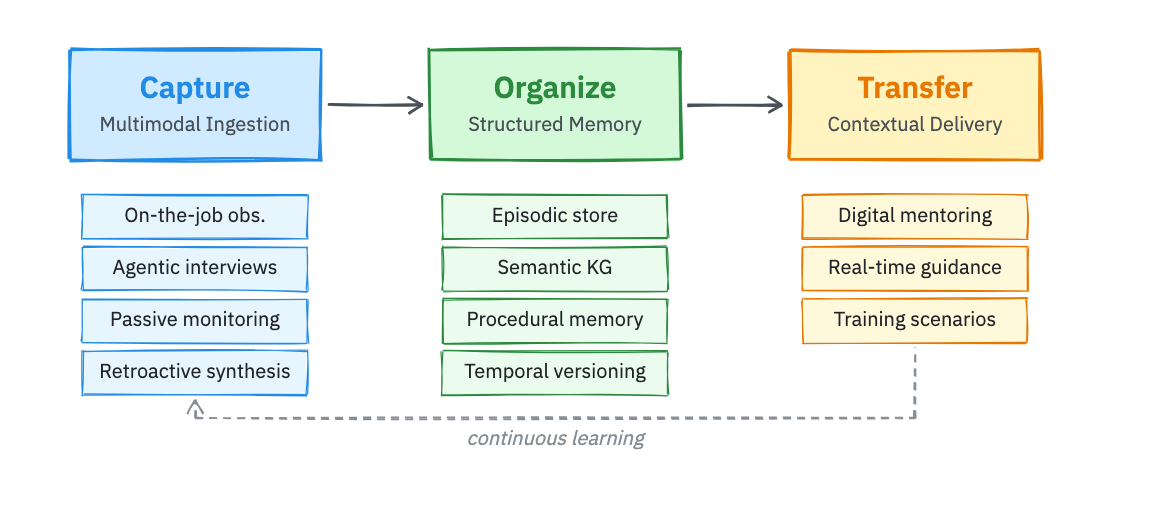
\includegraphics[width=\textwidth]{figures/tacit-pipeline.png}
\caption{The \textsc{Capture--Organize--Transfer} framework. A
  feedback loop enables the agent to refine its knowledge continuously
  from new worker interactions.}\label{fig:pipeline}
\end{figure}

\subsection{Stage 1: Capture---Minimally Invasive Multimodal
  Ingestion}\label{sec:capture}

A core design principle is minimal invasiveness. Experts are
scarce, busy, and cannot be pulled from the production floor for lengthy
knowledge-engineering sessions. The agentic system must capture
knowledge while experts work, combining multiple modalities. We identify an invasiveness spectrum ranging from fully passive
to lightly interactive, each targeting different knowledge layers:

\paragraph{Passive process mining (zero worker effort).}
Existing machine logs, shift records, and maintenance tickets contain
latent expert knowledge. Eschbach's Shiftconnector~\cite{eschbach2025} mines years of
accumulated shift logs to surface tacit patterns retroactively.
Explainable ML pipelines can differentiate expert from novice behavior
from process data alone with {>}90\% accuracy, requiring no worker
instrumentation~\cite{explainableml2024}. This layer captures
what experts do differently, but not the underlying decision process.

\paragraph{Ambient observation (no behavior change).} Computer
vision monitors expert actions during normal production; wearable eye
trackers reveal visual attention strategies that experts cannot
verbalize. Denso deployed Tobii eye-tracking glasses on inspectors,
uncovering gaze patterns that explained exceptional quality and halving
training time~\cite{tobii2025}. This layer captures embodied knowledge
that resists articulation---a partial answer to Polanyi's paradox.

\paragraph{Agentic micro-interviews (brief, contextual).} Rather
than lengthy sessions, the agent conducts brief elicitation at natural
pause points---shift changes, after anomaly resolution, or during
routine checks. The Bosch Shopfloor Agent, deployed at Bosch Bamberg,
uses a multi-agent system with voice interaction to diagnose root
causes from historical data, saving {\texteuro}850K per plant
annually~\cite{bosch2025}. Crucially, the agent asks rather
than only answers~\cite{najjar2025}, proactively filling
knowledge gaps.

\paragraph{Retroactive synthesis (automated, continuous).} The system continuously ingests
shift handoff notes, chat messages, and informal documentation, which
Uchihira~\cite{uchihira2026} calls ``digital fragmented
knowledge'', and links expert actions to contemporaneous sensor data,
capturing the physical context that triggered intervention.

The key distinction from existing approaches is that the capture agent
operates autonomously and continuously across all layers,
identifying what it does not know and opportunistically filling
gaps---rather than relying on scheduled documentation sessions.

\subsection{Stage 2: Organize---Temporally Versioned Structured
  Memory}\label{sec:organize}

Following the cognitive memory taxonomy~\cite{sumers2024coala}, captured
knowledge is organized into three interconnected, temporally versioned
stores (Table~\ref{tab:memory-arch}).

\paragraph{Episodic memory} stores specific situated events with full
context: who acted, what happened, when and where, what machine state
triggered the intervention, and what the outcome was. Each episode is
represented as a structured node carrying the tuple
$\langle$\textit{trigger, context, action, outcome, actor,
timestamp}$\rangle$, linked to contemporaneous sensor snapshots and
machine state vectors. This is the layer most critically absent from
current systems: no surveyed platform stores the situated event ``bearing
on Press~7 failed after weekend shutdown in high humidity and the senior
technician diagnosed misalignment, not wear'' as a retrievable,
contextually grounded episode. Architecturally, episodic stores require
graph-based representations where episodes connect to equipment nodes,
personnel, and environmental conditions, given that flat vector stores cannot
represent the relational structure of situated
events~\cite{graphmemsurvey2026}.

\paragraph{Semantic memory} consolidates abstracted knowledge into a
manufacturing knowledge graph grounded in domain ontologies (e.g.,
ISA-95 for process hierarchies, ISO~14224 for failure
classification). Nodes represent equipment, materials, failure modes, and
causal relationships; edges encode dependencies (``polymer~X requires
pressure $\leq$3.8\,bar'') and constraints. Crucially, semantic
nodes are derived from episodic evidence: the generalization
``weekend shutdowns increase bearing misalignment risk on hydraulic
presses'' emerges only after multiple episodes are consolidated.
This episodic-to-semantic consolidation mirrors how human experts build
intuition from accumulated experience~\cite{gam2026}.

\paragraph{Procedural memory} encodes how to perform tasks as
step sequences, decision trees, and conditional heuristics, including
experts' rules of thumb that deviate from official SOPs. Each procedure
carries version metadata and links to the episodic evidence from which
it was derived: ``Step~3 was added after the incident on 2024-03-15
(Episode~\#247).'' This provenance chain means procedures are not
opaque prescriptions but auditable, traceable instructions whose
rationale can be inspected, a requirement for safety-critical
manufacturing and EU AI Act compliance.

\paragraph{Bi-temporal versioning.}
All three stores must be temporally versioned using a
bi-temporal model~\cite{rasmussen2025} that distinguishes event
time, i.e. when something happened on the shop floor, from ingestion
time, i.e. when the system learned it. Every knowledge edge carries an
explicit validity interval. When a material substitution changes process
parameters, the old edge is closed and a new one opened, thereby preserving the
full history. This enables temporal queries that no current system
supports: ``What was the recommended pressure before the polymer
switch in March 2024?'' or ``When did we first learn that humidity
affects bearing alignment?''

\paragraph{Consolidation loop.}
A periodic consolidation process promotes recurring patterns from
episodic to semantic memory and distills validated action sequences into
procedural memory, while retaining the source episodes as provenance.
This mirrors the hierarchical consolidation formalized in recent memory
theory~\cite{timem2026}. Here, raw episodes are never discarded, but
increasingly abstract representations are layered on top, enabling
retrieval at the appropriate granularity, i.e. from a specific incident
(episodic) to a general principle (semantic) to an executable procedure
(procedural).

\subsection{Stage 3: Transfer---Contextual Delivery to New
  Workers}\label{sec:transfer}

The value of preserved knowledge is realized through effective transfer.
The agentic system supports three delivery modalities:

\paragraph{Digital mentoring.}
The agent acts as a virtual experienced
colleague, answering not just ``how'' but ``why'' by retrieving relevant
episodes (``The last time someone saw this vibration on Press\,7 after a
humid weekend, it was bearing misalignment and here's what the senior
technician did'');

\paragraph{Real-time guidance.}
In-ear or on-screen support calibrated
to the worker's experience level, from procedural steps (novices) to
contextual warnings (intermediates);

\paragraph{Scenario-based training.}
Past episodes recomposed into exercises that expose new workers to rare edge cases omitted from
official materials. Crucially, the feedback loop
(Figure~\ref{fig:pipeline}) ensures the knowledge vessel continues
learning from new workers' experiences, extending the knowledge base
beyond what any single expert contributed.


\section{Illustrative Walkthrough: Bearing Failure After Material
  Substitution}\label{sec:walkthrough}

To ground the framework concretely, we trace a representative
manufacturing scenario through all three stages. This walkthrough illustrates what no current system provides: the
connection between a situated episode, its temporal context, the
generalized knowledge derived from it, and the executable procedure
grounded in that evidence.

\paragraph{Scenario.} A hydraulic press (Press\,7) uses polymer seals
from Supplier\,A with a recommended operating pressure of 4.2\,bar. In
March~2024, procurement switches to Supplier\,B's polymer, which
requires lower pressure. Over subsequent months, a senior technician
discovers through trial and error that 3.8\,bar is optimal, and that
weekend shutdowns in humid conditions cause bearing misalignment (not
wear, as the maintenance manual suggests). In September, a partial
reversion to 4.0\,bar proves necessary due to batch variability. The
technician retires in December~2024.

\paragraph{Stage~1 (Capture)} The knowledge vessel captures this
expertise through multiple modalities: i)~passive mining
detects the pressure parameter change in machine logs and correlates it
with the supplier switch in procurement records; ii)~ambient
observation via vibration sensors flags anomalous bearing behavior
after weekend shutdowns; and iii)~an agentic micro-interview at
shift change, triggered by the anomaly, elicits the technician's
diagnosis: ``It's misalignment from thermal contraction, not wear.
Check alignment before you check the bearing.'' None of these modalities
alone captures the full picture; the agent synthesizes across all three.

\paragraph{Stage~2 (Organize)} The captured knowledge populates all
three memory stores:
Episodic: three distinct event nodes record the initial failure
(March), the humidity discovery (July), and the pressure reversion
(September), each linked to sensor snapshots and the technician's
explanations.
Semantic: the knowledge graph gains edges
\texttt{Polymer\,B}~$\xrightarrow{\text{requires}}$~\texttt{${\leq}$3.8\,bar}
with validity $[\text{Mar\,2024},\,\text{Sep\,2024})$ and
\texttt{Polymer\,B}~$\xrightarrow{\text{requires}}$~\texttt{4.0\,bar}
from $[\text{Sep\,2024},\,\text{now})$, plus a causal edge
\texttt{humid\_weekend}~$\xrightarrow{\text{causes}}$~\texttt{bearing\_misalignment}
on hydraulic presses.
Procedural: the restart checklist gains a new step: ``After
weekend shutdown in $>$60\% RH: verify bearing alignment before
production start (source: Episodes \#247, \#251).''

\paragraph{Stage~3 (Transfer)} Six months after the technician's
retirement, a new operator encounters unusual vibration on Press\,7
after a rainy weekend. The knowledge vessel retrieves the relevant
episodes and provides contextual guidance: ``Similar vibration was
diagnosed as bearing misalignment (not wear) by [senior technician]
in July~2024 under similar humidity conditions. Recommended action:
check alignment per Step~3a of the restart checklist. Historical
episodes: \#247, \#251.'' The operator follows the procedure, confirms
misalignment, and resolves the issue in minutes rather than hours. A
conventional SOP would have directed them to replace the bearing.

\begin{table}[h!]
\centering
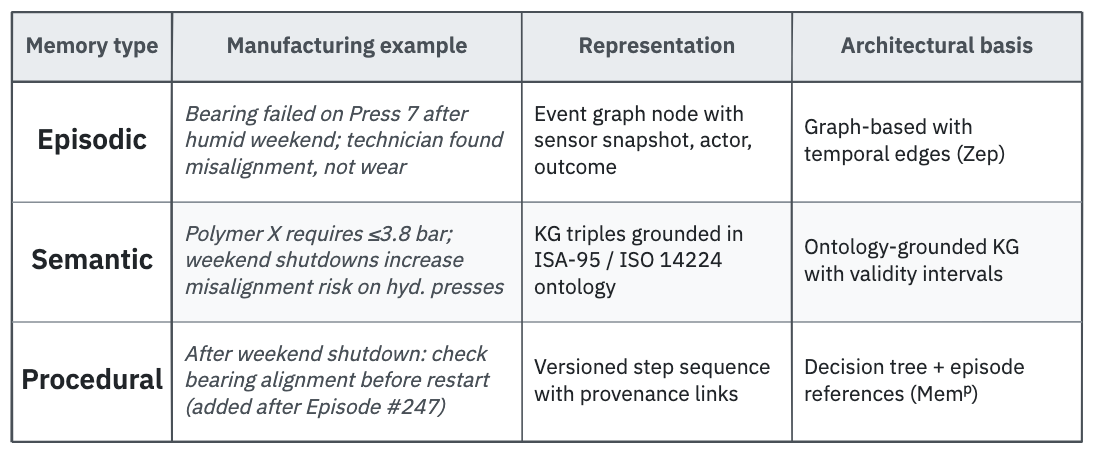
\includegraphics[width=\textwidth]{figures/tacit-memory-arch-table.png}
\caption{Architectural mapping: memory types, manufacturing knowledge,
  and realization. Each store is temporally versioned with bi-temporal
  validity intervals~\cite{rasmussen2025,memp2025}.}\label{tab:memory-arch}
\end{table}

\newpage

%%% ==================================================================
\section{Challenges and Open Questions: An Invitation to Discussion}\label{sec:discuss}
%%% ==================================================================

The architecture outlined above is deliberately a design
proposal, not a finished system. We identify six open challenges that
we believe warrant community discussion.

\paragraph{The boundary of the expressible.}
Polanyi's observation that ``we can know more than we can
tell''~\cite{polanyi1966} remains a fundamental constraint. AI can
capture expressible tacit knowledge, including heuristics, rules of thumb,
or decision rationales, but deeply embodied knowledge (the ``feel'' of a
machine vibration) resists formalization. Ambient sensing (eye tracking,
motion capture) can approximate the physical correlates of embodied skill
but cannot fully replicate the experience. \emph{Where exactly does the
boundary lie for manufacturing knowledge, and how should a system
communicate its own epistemic limits?}

\paragraph{The apprenticeship paradox.}
Ide~\cite{ide2026} formalizes a counterintuitive risk: AI systems that
reduce the need for human mentoring may weaken the
apprenticeship pipeline through which deep tacit knowledge is
transmitted. Our framework positions the agent as a complement to
human mentoring, which is consistent with the empirical finding that workers
prefer human experts when available~\cite{freire2024}. The analogy
of a digital apprentice is instructive: a novice standing next to
a master craftsman observes an action, thinks, and then asks ``did you
do that because\ldots?'' The master often would not have volunteered the
information unprompted and the question itself triggers externalization
of knowledge that would otherwise remain tacit. But the apprentice
cannot ask about everything; productive elicitation requires
knowing what one knows and what one does not, and formulating
questions intelligent enough to reach the relevant context.
An effective capture agent must implement this same metacognitive
cycle: maintain a model of its own knowledge gaps, generate targeted
hypotheses about expert behavior, and use those hypotheses to prompt
externalization. \emph{How do we design systems that strengthen rather
than substitute human knowledge transfer, and that elicit knowledge
the expert does not know they possess?}

\paragraph{The knowledge graph scope dilemma.}
A fundamental practical challenge concerns the boundary of what to
model. Consider a production anomaly: the root cause could be a supplier
change, a recipe modification, an operator intervention---or that the
climate control system was adjusted, subtly altering humidity in the
production hall. What should go into the knowledge graph when, in
principle, anything could be relevant? A data-lake approach
(ingest everything including environmental sensors, weather data, satellite
imagery, supplier records) maximizes the probability of later
discovery, but at explosive cost, and the vast majority of captured
data will never be queried. Conversely, a selective approach risks
omitting the one variable that explains an anomaly months later.
This is the unknown unknowns problem applied to knowledge
engineering: one cannot instrument what one does not anticipate
needing. Possible mitigation strategies include event-driven selective
ingestion, where anomalies automatically trigger broadened context
capture across adjacent data sources, and progressive graph expansion,
where the agent starts with a core ontology and expands it when
retrieved context proves insufficient for explanation.
\emph{What principles should govern knowledge graph scope in
manufacturing, and can agents learn to adaptively expand their own
ontologies?}

\paragraph{Is structured memory the right abstraction?}
A more fundamental question challenges the premise of our
architecture: given sufficiently capable models and sufficiently
comprehensive raw data, is explicit episodic-temporal structuring
actually necessary? If the agent has access to all raw sensor logs,
maintenance records, and production data, perhaps a sufficiently
large context window or retrieval-augmented generation over
unstructured data is enough---the model itself discovers the relevant
context without requiring pre-structured graphs. If so, the
episodic-temporal architecture we propose may be creating an
artificial bottleneck where the real limitation lies elsewhere, such
as in data access or model reasoning capacity. We believe structured
memory remains essential for three reasons: i)~manufacturing
knowledge spans years, far exceeding any context window;
ii)~temporal validity (``this parameter was correct before
the supplier switch'') requires explicit versioning that flat
retrieval cannot provide; and iii)~provenance chains from
procedures through episodes to raw data are necessary for
safety-critical auditability. Nevertheless, \emph{rigorous empirical
comparison between structured and unstructured memory approaches on
manufacturing knowledge tasks remains an open gap.}

\paragraph{Safety, governance, and trust.}
In safety-critical manufacturing, incorrect knowledge transfer can cause
physical harm. Memory poisoning has been identified as a top agentic
risk, with demonstrated injection rates exceeding
95\%~\cite{owasp2026}. The EU AI Act's high-risk provisions (applicable August 2026)
classify AI in safety-critical manufacturing as high-risk, mandating
transparency, human oversight, and tamper-evident audit trails.
\emph{What validation mechanisms are sufficient for graph-based memory
architectures in high-stakes environments? How should provenance and
temporal versioning interact with regulatory audit requirements?}

\paragraph{SME feasibility.}
The most acute knowledge concentration risk is in SMEs, where a single
retirement can eliminate critical capabilities. Lightweight, voice-first
interfaces, such as Murray Mentor's in-ear guidance~\cite{murraymentor2025} and Radhakrishnan's
BPMN capture~\cite{radhakrishnan2025}, demonstrate that
effective capture need not require heavy IT infrastructure. \emph{Can the
graph-based memory architecture we propose be realized in
resource-constrained settings, or does it inherently require
enterprise-scale infrastructure?}

\paragraph{Declaration of AI Use.}
This paper was prepared with the assistance of Claude (Anthropic) for
manuscript editing, proofreading, and bibliography formatting. All
intellectual content, analysis, and conclusions are solely the authors'.

%%% ==================================================================
\section{Conclusion}\label{sec:conclusion}
%%% ==================================================================

The manufacturing sector's tacit knowledge crisis is urgent, costly,
and accelerating. While commercial platforms address knowledge
capture, the entire field operates within a documentation
paradigm that discards the episodic, temporal, and situated qualities
that make expert knowledge most valuable. We have argued for reframing
tacit knowledge preservation as an agent memory problem and sketched the
\textsc{Capture--Organize--Transfer} architecture, in which graph-based
memory structures provide the unifying representation at every layer.
The gap we identify is actionable: agentic AI infrastructure and
manufacturing knowledge management both exist in mature form, but have
not yet been connected through an episodic-temporal memory architecture.
The challenges outlined define a concrete
research agenda, from the epistemic boundaries of capture, through
the scope and structural adequacy of graph-based memory, to governance
and SME feasibility. While this paper focuses on manufacturing, the
reframing may generalize to any domain facing tacit knowledge loss,
including healthcare, skilled trades, and engineering. We invite the
community to engage with these challenges and to collaboratively
advance memory-grounded knowledge preservation.

%%% ==================================================================
%% Bibliography
%%% ==================================================================

\begin{thebibliography}{41}

\bibitem{apqc2025} APQC: Knowledge exodus from the silver tsunami in
  the industrial products sector: It is AI or bust. ATD Blog (2026)

\bibitem{hu2025survey} Hu, Y., et al.: Memory in the age of AI agents:
  A survey. arXiv:2512.13564 (2025)

\bibitem{bosch2025} Bosch: Agentic AI in manufacturing
  production---Shopfloor Agent. Bosch Stories (2025)

\bibitem{cogniman2025} Belbachir, A., et al.: COGNIMAN digital twin
  architecture for flexible manufacturing. J.\ Intell.\ Manuf.\ (2025)

\bibitem{deloitte2024} Deloitte, NAM: Creating pathways for tomorrow's
  workforce today. Manufacturing Institute Report (2024)

\bibitem{dovient2025} Dovient: The real cost of tribal knowledge loss
  in manufacturing. White Paper (2025)

\bibitem{edwards2026} Edwards, K.M., et al.: Agentic AI in engineering
  and manufacturing. arXiv:2604.09633 (2026)

\bibitem{egain2025} eGain: Capturing tacit knowledge from the great
  retirement cohort using GenAI. Report (2025)

\bibitem{explainableml2024} de~Arriba-P\'erez, F., et al.: Automatic
  generation of insights from workers' actions in industrial workflows
  with explainable Machine Learning. arXiv:2406.12732 (2024)

\bibitem{fortune2026} Sharma, K.: Let's train workers on industrial AI,
  not replace them. Fortune (Jan 2026)

\bibitem{freire2024} Kernan~Freire, S., et al.: Knowledge sharing in
  manufacturing using LLM-powered tools. Frontiers in AI \textbf{7}
  (2024)

\bibitem{horizon2027} European Commission: Horizon Europe Work Programme
  2026--2027, Topic HORIZON-CL4-2027-02-DIGITAL-EMERGING-52: New
  approaches for Human/AI collaboration (2026)

\bibitem{ide2026} Ide, E.: Automation, AI, and the intergenerational
  transmission of knowledge. arXiv:2507.16078 (2025)

\bibitem{kieeper2025} Ottersb\"ock, N., et al.\ (eds.):
  Wissensmanagement mit K\"unstlicher Intelligenz. Springer (2025)

\bibitem{najjar2025} Najjar, R.: From AI-based KM assistant to tacit
  knowledge agent: Leveraging small language models for tacit knowledge
  extraction. Medium (2025)

\bibitem{owasp2026} OWASP: Agentic security initiative---ASI06: Memory
  poisoning. OWASP Foundation (2026)

\bibitem{panopto2018} Panopto: Workplace knowledge and productivity
  report (2018)

\bibitem{polanyi1966} Polanyi, M.: The Tacit Dimension. Univ.\ of
  Chicago Press (1966)

\bibitem{radhakrishnan2025} Radhakrishnan, U.: Documenting SME processes
  with conversational AI. arXiv:2512.05122 (2025)

\bibitem{sumers2024coala} Sumers, T.R., et al.: Cognitive architectures
  for language agents. Trans.\ Mach.\ Learn.\ Res.\ (2024)

\bibitem{tobii2025} Tobii: Unlocking hidden skills---eye tracking for
  workforce training. Tobii Blog (2025)

\bibitem{uchihira2026} Uchihira, N.: Tacit knowledge management with
  generative AI: The GenAI SECI model. arXiv:2603.21866 (2026)

\bibitem{zuin2025} Zuin, G., et al.: Leveraging LLMs for tacit
  knowledge discovery. IJCNN (2025)

\bibitem{graphmemsurvey2026} Yang, C., et al.: Graph-based agent
  memory: A survey. arXiv:2602.05665 (2026)

\bibitem{gam2026} Wu, Z., et al.: GAM: Hierarchical graph memory for
  LLM-based agents. In: ICLR 2026

\bibitem{rasmussen2025} Rasmussen, P., et al.: Zep: Temporal knowledge
  graph for agent memory. arXiv:2501.13956 (2025)

\bibitem{timem2026} TiMem: Temporal-hierarchical memory consolidation
  for language agents. arXiv:2601.02845 (2026)

\bibitem{memp2025} Fang, R., et al.: Mem$^{\mathrm{p}}$: Exploring
  agent procedural memory. arXiv:2508.06433 (2025)

\bibitem{destatis2025} Statistisches Bundesamt: 13.4 Millionen
  Erwerbspersonen \"uberschreiten bis 2039 das Rentenalter. Destatis
  Press Release N048 (2025)

\bibitem{iwkoeln2025} Sch\"afer, H., Deschermeier, P.: Fast 20
  Millionen Erwerbst\"atige gehen bis 2036 in Rente. IW K\"oln (2025)

\bibitem{zdh2025} Zentralverband des Deutschen Handwerks:
  Fachkr\"aftemangel und Betriebsnachfolge im Handwerk. ZDH (2025)

\bibitem{bitkom2026} Bitkom: KI-Einsatz in der deutschen Wirtschaft.
  Bitkom KI-Studie (2026)

\bibitem{murraymentor2025} Murray Mentor: Voice-first AI guidance for
  industrial frontline workers. Murray Mentor (2025)

\bibitem{blockbrain2026b} Blockbrain: Digital knowledge twins---responsible
  AI agents against company knowledge loss. Blockbrain AG Press Release
  (2026)

\bibitem{augmentir2025} Augmentir: AI-powered connected worker platform
  for manufacturing. Augmentir Inc.\ (2025)

\bibitem{maintainx2025} MaintainX: Connected worker platform for
  industrial maintenance and operations. MaintainX Inc.\ (2025)

\bibitem{poka2025} Poka: Connected worker platform for manufacturing
  knowledge sharing. Poka Inc.\ (2025)

\bibitem{siemensifm2025} Siemens: Industrial Copilot powered by the
  Siemens Industrial Foundation Model. Siemens AG (2025)

\bibitem{sapcompanymemory2025} SAP: Joule with Company
  Memory---enterprise knowledge context graph. SAP SE (2025)

\bibitem{ibmmaximo2025} IBM: Maximo Application Suite with watsonx.ai
  for intelligent asset management. IBM (2025)

\bibitem{eschbach2025} Eschbach: AI-powered knowledge transfer in
  manufacturing with Shiftconnector Smart Search. CHEManager (2025)

\bibitem{fraunhoferiese2025} Fraunhofer IESE: AI-supported modeling and
  knowledge transfer. Fraunhofer IESE, Dept.\ Embedded Systems
  Engineering (2025)

\bibitem{dihk2025} DIHK: Fachkr\"aftereport 2025/2026:
  Fachkr\"afteengp\"asse bleiben Herausforderung. Deutsche Industrie-
  und Handelskammer (2025)

\end{thebibliography}

\end{document}
